\chapter{Materiales y Metodos}
Las técnicas de relevamientos transcripcionales de gran escala, tales como las micromatrices de ADN y secuenciamientos de ARN (secuenciadores de próxima generación), permiten el monitoreo en paralelo de la totalidad del genoma. En este capítulo daremos una introducción al funcionamiento del primer tipo de tecnologías, que será la que usaremos extensivamente en este trabajo, y a los diferentes conjuntos de datos que utilizaremos.\cite{Bose2016}

\section{Micromatrices de ADN}
La tecnología de micromatrices de ADN se constituyó como una herramienta indispensable para el monitoréo de niveles de expresión a lo largo de todo el genoma de un organismo, estimando la concentración de ARNm que está siendo exportado desde el núcleo celular hacia el citoplasma para la síntesis de determinadas proteínas.\\
Una micromatriz es típicamente un portaobjetos de vidrio u otra superficie sólida a la cual se le adosan de forma ordenada y en lugares específicos (llamados sondas) moléculas de ADN. Un mismo sitio puede contener varios millones de copias de moléculas idénticas de ADN de composición conocida (tanto genómico como hebras cortas de oligo-nucleótidos) que se corresponden de forma unívoca con un gen. Una micromatriz de ADN puede medir en simultaneo los niveles de expresión de hasta 40000 genes distintos.\\
Dependiendo de la tecnología utilizada, las micromatrices pueden ser de canal único o de doble canal.\\
\begin{figure}[h]
    \centering
    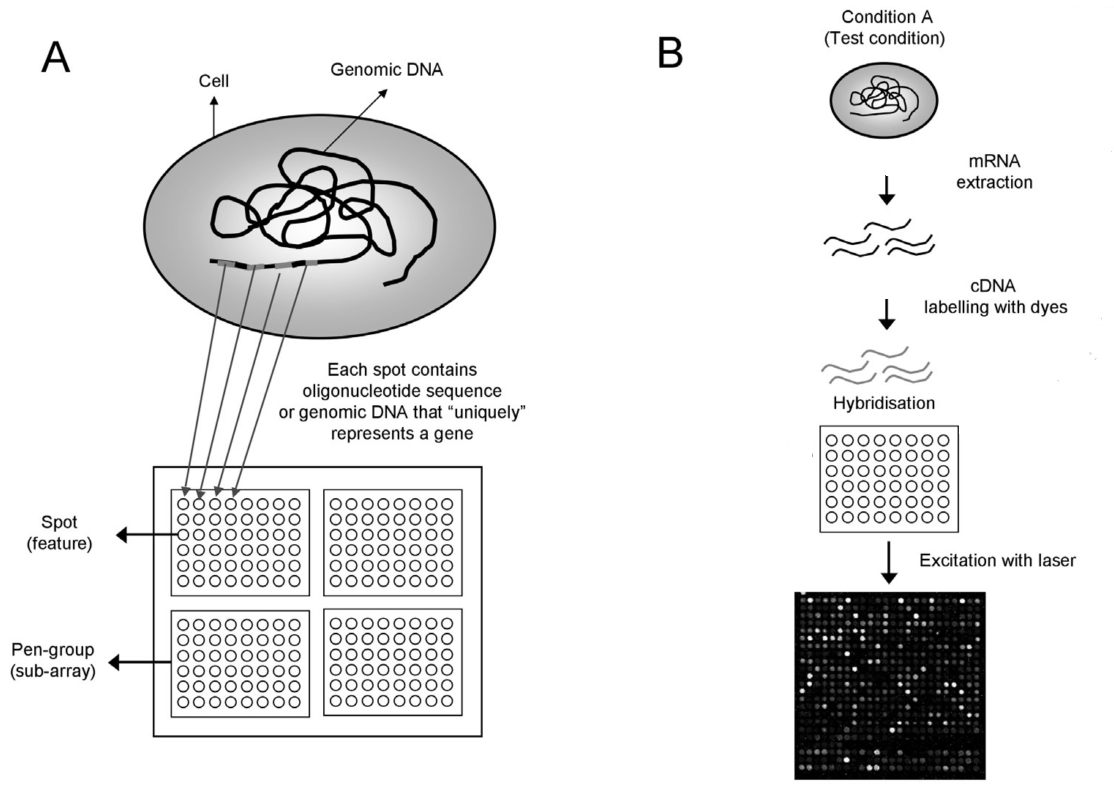
\includegraphics[width=0.8\textwidth]{micromatriz}
    \caption{Funcionamiento básico de una micromatriz de ADN \hl{Hacer esta figura nuevamente}}
    \label{fig:micromatriz}
\end{figure}
En las micromatrices de un solo canal, las moléculas de ARNm son extraídas de las células de interés del organismo y mediante diversas técnicas son transcritas inversamente a ADN. Luego, el ADN es transcrito nuevamente a ARNm utilizando ARN marcado con un compuesto fluorescente (biotina). Estas copias marcadas y aumentadas son luego colocadas en la micromatriz, permitiendo que el ARNm se difunda por toda la misma.\\
Cuando el ARNm encuentra una sonda que contiene su copia complementaria, se hibridiza con la misma, es decir se pega con una afinidad mucho mayor con la que se puede pegar a cualquier otra. Al lavarse la solución de ARNm, solo aquellos que se hibridizaron con la copia complementaria se mantienen unidos. Finalmente, se ilumina la micromatriz con luz laser de longitud adecuada y se mide la cantidad de fluorescencia emitida por cada sonda. Esta cantidad está asociada a la cantidad de ácido nucléico que se ligó a una dada sonda y eso a su vez será proporcional a la concentración de ese ARNm particular en el tejido de interés.\\
El resultado de un experimento con micromatrices es una tabla o matriz de expresión de $N_g x N_m$ donde cada fila corresponde a los niveles de expresión de cada gen particular ($N_g \approx 20000$ genes), y cada columna a cada muestra ($N_m \approx 15$ muestras) de tejido tomada.\\
Estos tecnologías plantean entonces el problema de como analizar bastas cantidades de datos para obtener información de interés, como ser:
\begin{enumerate}
	\item La identificación de los genes que forman parte de algún proceso biológico
	\item Agrupar tumores para su clasificación clínica
	\item Proveer evidencia de la función de proteínas cuyo rol en el organismo se desconoce
\end{enumerate}
En la actualidad, la aparición de tecnologías más rápidas y económicas de secuenciamiento, conocidas colectivamente como Next-generation sequencing (Secuenciamiento de próxima generación), están comenzando a dejar obsoleta la tecnología de micromatrices. Sin embargo, las mismas siguen siendo una herramienta útil en el estudio de los perfiles de expresión genética.\\
En este trabajo, analizaremos el conjunto de datos Wiegel, datos obtenidos mediante esta tecnología.\cite{Babu2004,Schulze2001,Domany2003}
\section{Conjunto de datos Wiegel}
En el marco del proyecto AtGenExpress, (un esfuerzo multinacional desarrollado para descubrir el transcriptoma del organismo modelo multicelular Arabidopsis thaliana), el grupo \textit{Weigel \& Lohmann}, de Alemania, realizó en el año 2004 un exhaustivo estudio de expresión del transcriptoma de Arabidopsis thaliana utilizando las micromatrices de ADN Affymetrix ATH1, con el objetivo de comprender las complejas redes de genes que, se conjetura, controlan la tolerancia de la planta al estrés. Para ello, se sometió a plantas de Arabidopsis, de idéntico genotipo y de idénticas condiciones de crecimiento, a diversos tratamientos de estrés.\\
Los tratamientos de estrés se realizaron de tal forma de excluir efectos circadianos (oscilaciones de las variables biológicas en intervalos regulares de tiempo asociadas con un cambio ambiental rítmico), tomando muestras o de la raiz (root) o del tallo (shoot) en dos réplicas biológicas cada 0 minutos, 30 minutos, 1 hora, 3 horas, 6 horas, 12 horas y 24 horas luego del comienzo del tratamiento. En algunos de los tratamientos, por ejemplo, de luz ultravioleta, las alteraciones transcripcionales producto del estrés son fueron tan rápidas que se tomaron además muestras a los 15 minutos del comienzo  del mismo. Las muestras de control se tomaron de plantas no sometidas a ningún tratamiento de estrés de la misma forma que con las plantas tratadas.\\
Además de un tratamiento de control, se realizaron los siguientos tratamientos de estrés:
\subsubsection*{Tratamiento de frío}
Las cajas conteniendo las plantas fueron transferidas a hielo para un rápido enfriamiento y mantenidas a 4\degree C en un cuarto frío hasta la cosecha.
\subsubsection*{Tratamiento de calor}
Las cajas fueron transferidas a una incubadora y sometidas a una temperatura de 38\degree C durante 3 horas antes de la cosecha.
\subsubsection*{Tratamiento osmótico y de sal}
Se removieron las balsas de polipropileno que sostienen a las plantas y se agregaron a la solución acuosa, mannitol y NaCl en na concentración final de 300 mM y 150 mM respectivamente. Luego, se devolvieron las balsas a su lugar hasta la cosecha.
\subsubsection*{Tratamiento de heridas}
Se hirió a las plantas utilizando un elemento punzante consistente en 16 agujas, tres veces por hoja, dejando en promedio entre 3 y 4 agujeros.
\subsubsection*{Tratamiento de sequía}
Las plantas fueron expuestas a una corriente de aire durante 15 minuto, lapso durante el cual perdieron un 10\% de su peso. Luego, se las devolvió a la cámara de cultivo hasta la cosecha.
\subsubsection*{Tratamiento con luz ultravioleta B}
Se irradió a las plantas durante 15 minutos con luz ultravioleta B. Bajo estas condiciones se induce una respuesta de la planta tanto para daño por radiación de onda corta como para radiación ultravioleta.

Además de estos tratamientos, se sometió de forma similar a tratamientos oxidativos, de genotoxicidad y de calor y recuperación.
\hl{en el paper no figura la informacion de los tratamientos de genotoxic, oxidative y heat and recovery}
\cite{AtGenExpress, Kilian2007}
\section{PIN - Redes de interacción de proteínas}
\label{sec:redes}
Las redes son construcciones útiles para esquematizar la organización de las interacciones en distinto tipo de sistemas. Las redes permiten tener una vision global de como estan organizadas dichas interacciones.\\
La mayor parte de las funciones biológicas en una célula es llevada a cabo por proteínas a través de procesos de interacción fisica entre ellas, por ejemplo formando complejos proteicos. Por lo tanto, es de fundamental importancia conocer no solo los niveles de expresión de una dada proteína, sino también, en simultaneo, las interacciones que lleva a cabo con otras proteínas. El registro en forma global de estas interacciones conforma lo que se denomina red de interacción de proteínas o PIN, y si la misma contempla la totalidad de las proteínas de una dada especie, la PIN correspondiente se conoce como interactoma completo.\\
\subsection{PIN AI1 y LCI binaria}
A lo largo de esta tesis se analizaron dos redes de interacción de proteínas con el objetivo de utilizarlas como referencia.\\
La primera, una red binaria de interacción de proteínas en todo el proteoma para la planta \textit{Arabidopsis thaliana} consistente en aproximadamente 5700 interacciones altamente confiables entre alrededor de 2700 proteínas, obtenida de \cite{Hahn2013}, material suplementario, tabla 4.\\
Para generar el interactoma, \cite{Hahn2013} utilizó una colección de aproximadamente 8000 marcos abiertos de lectura (secuencias de ARN comprendidas entre un codón de inicio de traducción y un codón de terminación) representando alrededor del 30\% de los genes codificantes. Probaron todas las interacciones de a pares con un método conocido como \textit{Sistema de doble híbrido} (Y2H por sus siglas en inglés), consistente en la activación de un gen reportero mediante la acción de un factor de transcripción sobre la secuencia regulatoria. Para ello, el factor de transcripción es separado en dos fragmentos, uno que reconoce la secuencia regulatoria y otro que promueve la activación de la transcripción. Estos dos fragmentos son luego conectados cada uno a cada una de las dos proteínas (llamadas carnada y presa) que se desean analizar. Si las dos proteínas interactúan entre si, el factor de transcripción se reconstituirá y se activará el gen reportero, visualizándose como crecimiento en un medio específico o una reacción con cambio de color.\cite{Bruckner2009}\\
Utilizando los pares obtenidos confeccionaron un conjunto de datos consistente en 5664 interacciones binarias entre 2661 proteínas, llamado Arabidopsis Interactome versión 1 ``main screen'', que llamaremos AI1.\\
\begin{figure}[h]
    \centering
    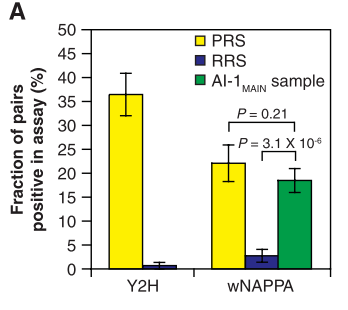
\includegraphics[width=0.4\textwidth]{calidad_ai1}
    \caption{Quality of AI-1MAIN.(A) Fraction of PRS, RRS, or AI-1MAIN sample pairs positive in Y2H or in wNAPPA at a scoring threshold of 1.5. Error bars, standard error of the proportion. P values, one-sided two-sample t tests (3). \hl{Ver si se puede poner esta figura, ver el epigrafe y como citarla}}
    \label{fig:calidad_ai1}
\end{figure}
La calidad de la red fue evaluada contra un conjunto de referencias positivas de 118 interacciones bien documentadas (PRS) y comparadas con un conjunto de referencia de 146 pares aleatorios de proteínas(RRS). Determinaron mediante la técnica de comparación \textit{wNAPPA}, que la fracción de interacciones reales en AI1, es decir su precisión, era de alrededor de 80\%, figura \ref{fig:calidad_ai1}. Esto implica que la red AI1 es una red de interacción de proteínas de alta calidad.\\
La segunda red utilizada fue una red binaria de interacción de proteínas, que llamaremos, $LCI_{binaria}$, obtenida de \cite{Hahn2013}, material suplementario, tabla 4, consistente en aproximadamente 4300 interacciones entre alrededor de 2200 proteínas de \textit{Arabidospis}. La misma fue obtenida mediante curado manual de literatura, es decir, en lugar de realizar ensayos de alto rendimiento en busca de pares de proteínas interactuantes, se realiza una revisión exhaustiva de la literatura existente en busca de interacciones que aparezcan en ensayos de pequeña escala previamente realizados sobre pocas proteínas y motivados por hipótesis previas (hypothesis-driven en inglés), ensayos altamente fiables.\cite{Cusick2009}\\
El solapamiento observado entre ambas se encuentra en el rango esperado dado la cobertura del proteoma que hacen estas redes, como muestra el diagrama de la figura \ref{fig:ai1_lci}.
\begin{figure}[h]
    \centering
    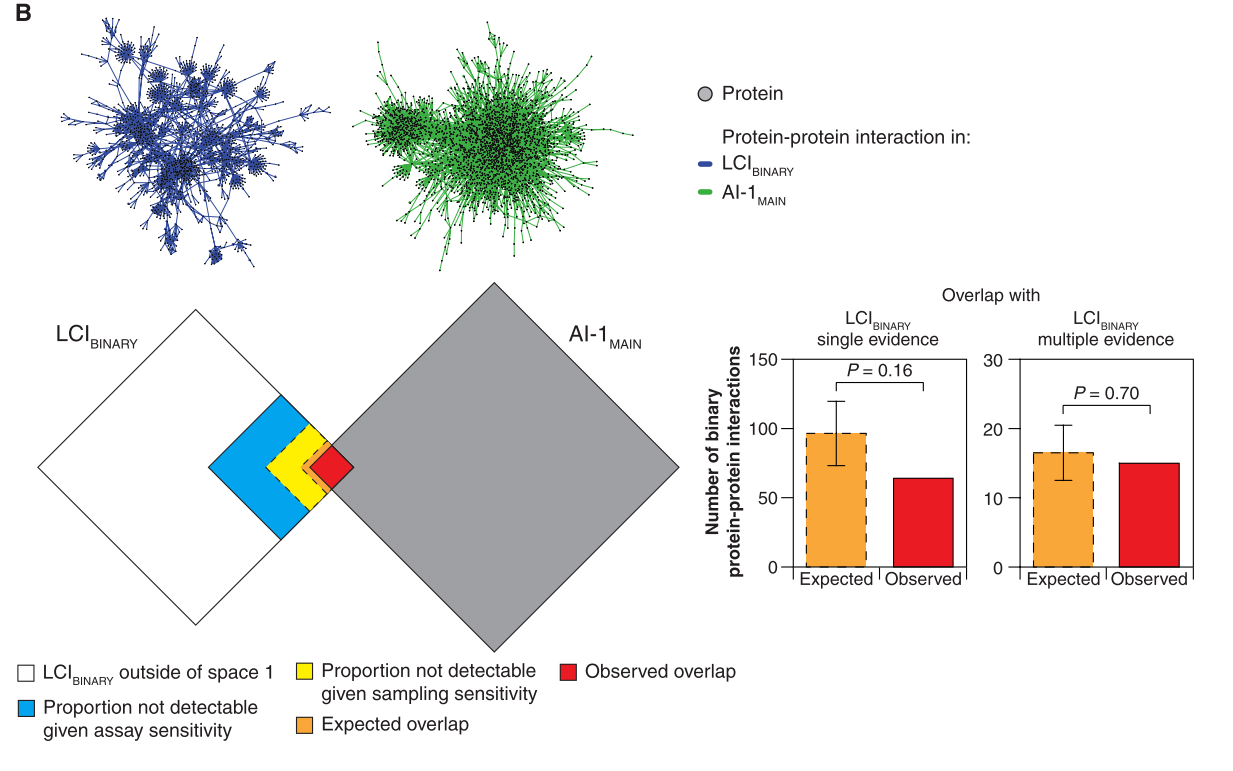
\includegraphics[width=0.8\textwidth]{ai1_lci}
    \caption{The number of literature-curated interactions recovered reflects AI-1MAIN framework parameters (6). (Top) Network rep- resentations of LCIBINARY and AI-1MAIN. (Bottom left) Data sets are represented by squared Venn diagrams; size is proportional to the number of interactions (3). (Bottom right) Observed and expected overlap given sensitivity and completeness of AI-1MAIN with LCIBINARY interactions supported by a single or multiple experimental evidences (3). PRS pairs were removed from LCIBINARY multiple evidence for this analysis. Error bars, two SD from the expected counts \hl{Ver si se puede poner esta figura, ver el epigrafe y como citarla}}
    \label{fig:ai1_lci}
\end{figure}
\section{KEGG - Vías metabólicas}
Los procesos celulares son llevados a cabo a través de interacciones entre varios genes y proteínas. Este tipo de actividades suele organizarse en vías, llamadas vías metabólicas, que consisten en grupos de genes que se coordinan para realizar una tarea específica. Son cadenas de reacciones bioquímicas que conducen de un sustrato inicial a uno o más productos finales. Descubrir este tipo de organizaciones es fundamental para obtener una imagen global de la actividad celular (figura \ref{fig:mapa_kegg}).\\
La Enciclopedia de Genes y Genomas de Kyoto (KEGG, por sus siglas en inglés), es una base de datos de recursos que comprenden funciones de alto nivel y utilidades de sistemas biológicos, como las células, los organismos y los ecosistemas, obtenida mediante información de nivel molecular generada por secuenciamientos de genoma y otros ensayos de gran escala. 
\begin{figure}[h]
    \centering
    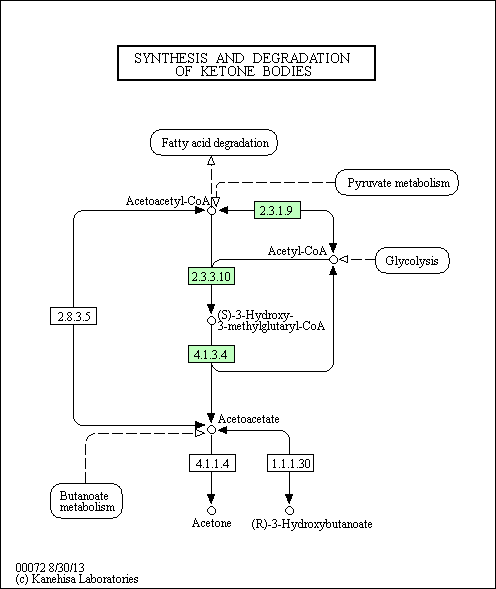
\includegraphics[width=0.8\textwidth]{mapa_kegg}
    \caption{Mapa KEGG de la vía metabólica de Arabidopsis Thaliana  \textit{Synthesis and degradation of ketone bodies} \hl{comentar mas o cambiar el idioma del grafico}}
    \label{fig:mapa_kegg}
\end{figure}
La misma provee de una base de datos de vías metabólicas que contiene recursos para la representación de procesos celulares tales como el metabolismo, transducción de señales y ciclo celular. En este trabajo utilizamos la base de datos KEGG de vías metabólicas de la planta \textit{Arabidospsis thaliana} disponible a través del paquete ``graphite'' (GRAPH Interaction from pathway Topological Environment) del lenguaje de programación R.\\
Se conformó una red uniendo todas las vías metabólicas presentes en la base de datos y teniendo en cuenta solamente aquellos genes presentes en el conjunto de datos Weigel.
\cite{Segal2003}\cite{Kanehisa2000}
\section{GO - Ontología genética}
Poder comparar y clasificar entidades es un mecanismo fundamental de las ciencias biológicas. El advenimiento de tecnologías de alta salida como las micromatrices de ADN, hace que sea necesario adoptar sistemas de representación del conocimiento que sean objetivos y estandarizados. Esto llevó al desarrollo de diversas ontologías para anotación de genes y de sus productos, y en particular, al desarrollo de la Ontología Génica (Gene ontology, GO por sus siglas en inglés).
El proyecto de Ontología Génica (GO) es un esfuerzo colectivo que intenta mantener un vocabulario y una descripción consistente de productos génicos a lo largo de distintas bases de datos. Esta ontología provee de un vocabulario controlado de términos definidos que representan las propiedades de los productos génicos (proteínas y secuencias de ARN, por ejemplo).\\
El proyecto GO consta de tres ontologías estructuradas que describen los productos génicos en terminos de sus procesos biológicos asociados (ontología \textit{Biological Process}, BP), de sus componentes celulares (ontología \textit{Cellular Component}, CC) y de sus funciones moleculares (ontología \textit{Molecular Function}, MF).\\
Un termino de un proceso biológico (BP) describe una serie de eventos realizados por uno o varios grupos de eventos moleculares con un comienzo y un fin definidos, por ejemplo, ``proceso celular fisiológico'' o ``transducción de señal''. Un proceso biológico no es equivalente a una vía metabólica ya que no intenta representar la dinámica o dependencias de la misma.\\
Un término de componente celular (CC) describe un componente de una célula que es parte de un objeto mayor, como ser una estructura anatómica (por ejemplo, retículo endoplasmático rígido, núcleo, etc.) o un grupo de productos génicos (por ejemplo, ribosoma, proteasoma, etc.).\\
Finalmente, los términos de función molecular (MF) describen las actividades que ocurren a nivel molecular, por ejemplo, ``actividad catalítica'' o ``actividad de transporte''.\\
La ontología GO está estructurada en tres grafos acíclicos dirigidos (DAG por sus siglas en inglés) independientes (uno para cada categoría ortogonal de productos génicos), donde cada nodo representa un término que describe alguna función. Los términos se unen entre si mediante relaciones del tipo ``es un'' o ``es parte de'', donde el primero expresa una relación de clase-subclase y el segundo una relación de parte-todo (figura \ref{fig:ejemplo_de_go}). Cuando un producto génico es descrito por un termino GO, se dice que el mismo está anotado en ese término, ya sea de forma directa o a través de herencia, ya que estar anotado en un término implica estar anotado en todos los términos ancestrales, regla conocida como \textit{regla del camino verdadero}.\\
\begin{figure}[h]
    \centering
    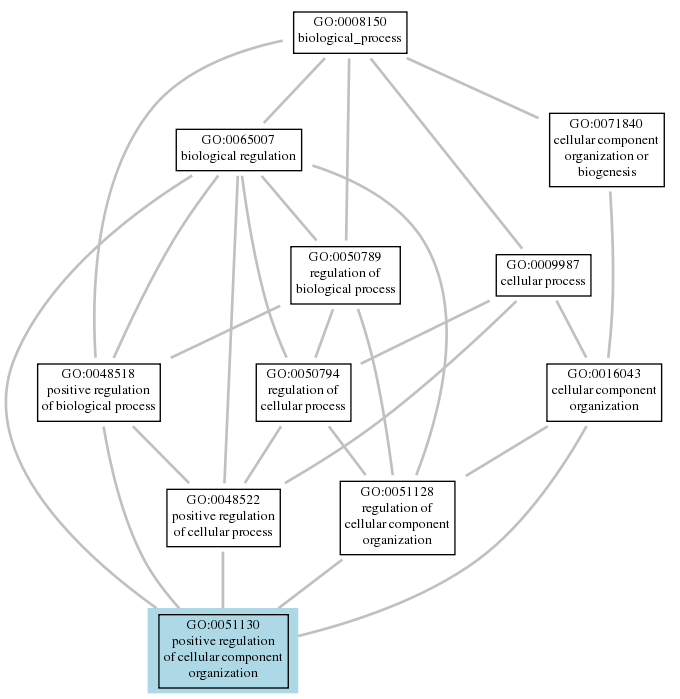
\includegraphics[width=0.5\textwidth]{ejemplo_de_go}
    \caption{Subgrafo mostrando el proceso biológico "Positive regulation" etc. \hl{poner nombres en castellano, flechas, etc}}
    \label{fig:ejemplo_de_go}
\end{figure}
Formalmente, podemos describir estás relaciones de la ontología GO de la siguiente manera:\\
Sea $C=\{c_i / 1\leq i \leq N\}$ un conjunto ordenado finito de conceptos que representan términos GO. Los mismos se relacionan entre si a través de las relaciones antes consignadas, de tal forma que $c_i \rightarrow c_j$ denota que $c_i$ es un/es parte de $c_j$. Basado en esto, es posible definir una relación binaria sobre $C$, denotada por $\preceq$, tal que $c_i \preceq c_j$, es decir $c_j$ es un ancestro de $c_i$ en la jerarquía GO. Notar entonces que si $c_k \preceq c_i$ y $c_i \preceq c_j \Rightarrow c_k \preceq c_j$ (regla del camino verdadero). En cada grafo existe un término raíz de la jerarquía $r$, tal que $c_i \preceq r \forall c_i \in C$.\\
Los conceptos más generales se hallarán más próximos al término raíz, mientras que los más específicos e informativos se alejarán del mismo. La anotación de un gen o producto génico se realiza siempre al nodo mas especifico, pudiendo ser anotado además en varios conceptos biológicos a la vez.\\
Una anotación en GO consiste en un término GO junto con una referencia que describe el tipo de trabajo o análisis que se realizó para asociar un gen con un término específico. Cada anotación debe además incluir un código de evidencia que indica la forma en que se justifica la anotación a un término particular, lo que le confiere un grado de fiabilidad.\\En particular, existen dos grupos de anotaciones, aquellas que fueron curadas manualmente y aquellas que fueron inferidas de anotaciones electrónicas (IEA). Este último tipo de anotaciones funcionales se realiza de forma automatizada sin que intermedie un curador e involucran comparaciones por similitud de secuencia o anotaciones transferidas de bases de datos y por lo tanto poseen una baja calidad y una gran cobertura, formando alrededor del 40\% de las anotaciones totales. Además, dentro del grupo de las anotaciones que fueron curadas manualmente, se tienen aquellas que fueron inferidas por medio de experimentos (IDA, IEP, IGI, IMP, IPI), aquellas que fueron inferidas por medio de análisis computacional (IBA, ISS, RCA, ISM). La figura \ref{fig:codigos_de_evidencia} muestra la fracción que representa cada tipo de anotación para cada ontología.
\begin{figure}[h]
    \centering
    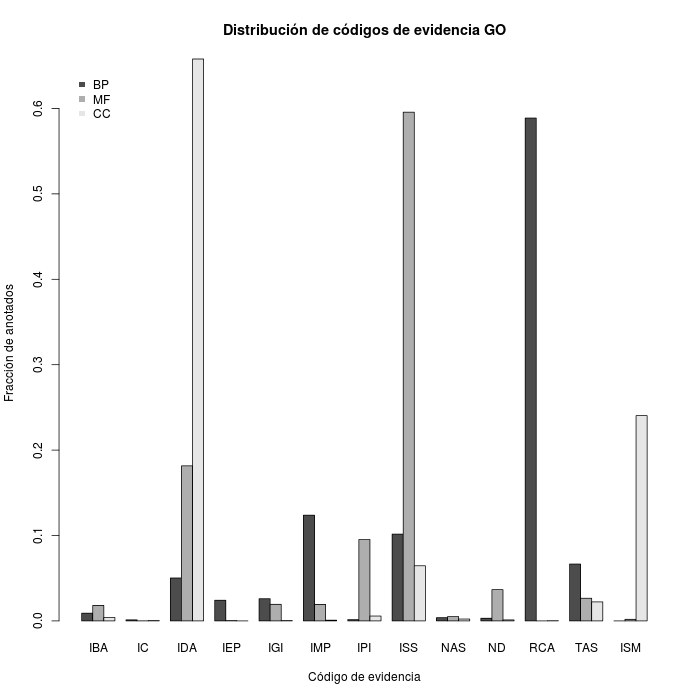
\includegraphics[width=0.8\textwidth]{codigos_de_evidencia}
    \caption{Códigos de evidencia en cada una de las ontologías y la fracción del total que representan. \hl{comentar mas}}
    \label{fig:codigos_de_evidencia}
\end{figure}
Las cantidad total de anotaciones para BP, MF y CC, sin tener en cuenta aquellas pertenecientes a la categoría IEA, totalizan 2540816, 207087 y 1043851 anotaciones respectivamente.\\
En particular, en este trabajo se tuvieron en cuenta únicamente las evidencias obtenidas experimentalmente. Para ello, se tomaron dos subconjuntos de anotaciones de la ontología BP, que llamaremos BPA, consistente en las anotaciones IDA, IPI, IGI, IMP, con un total de 512235 anotaciones y BPB, consistente en las anotaciones IDA, IPI, IGI, IMP y IEP, con un total de 573688. Además, se utilizó un subconjunto de la ontología CC, consistente en las anotaciones IDA, IPI, IGI, IMP, con un total de 693991 anotaciones.\cite{Pandey2008} \cite{Resnik1995} \cite{Bose2016} \cite{Pesquita2009} \cite{Berenstein2014} \cite{Ashburner}
